%!TEX program = XeLaTeX
%!TeX root =main.tex
%请在下面输入本章内容。
\section{文献的引用} \label{sec:Ref}
论文文本中需要引用参考文献来注明出处。

\subsection{在文本中的引用方式} \label{ssec:Txtref} %
引用可分为作为文章内容的普通引用,和只作为注解用的上标引用。

\subsubsection{普通引用} \label{sssec:Tcite} %
引用方式\cite{Designated}为普通引用。

\subsubsection{上标引用} \label{sssec:Tupcite}
有时候还需要用到上标引用\upcite{jiyulisanduishu,cyu282}。

\subsection{在图表中的引用方式} \label{ssec:PnTref}
图表中亦可引用文献,方法与文本中引用相同(见$\S$ \ref{ssec:Txtref})。

\begin{figure}[!ht]
  \centering
  % Requires \usepackage{graphicx}
  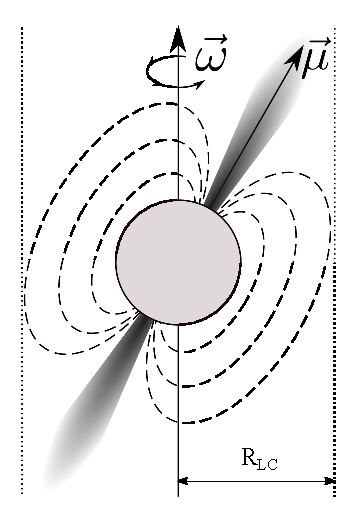
\includegraphics[width=.3\textwidth]{img/lighthouse.eps}\\
  \caption{此处可以引用文献 \upcite{yang_nulling_2014}。}\label{fig:Lighthouse}%{Cooling curve of Pulsars}
\end{figure}


\subsection{小结}
以上为本模板的文献引用方式。
